\begin{surferIntroPage}{Tutorial}{tutorial_koord1}{Prvi koraci sa SURFER-om}
Naziv ove aplikacije je SURFER. Ime SURFER nas odmah podsje\' ca na more, sunce i valove, ali u ovom slu\v caju ime SURFER dolazi od engleske rije\v ci {\it surface}, \v sto ozna\v cava plohu.
\\
Koriste\' ci SURFER mo\v zemo prikazati razne plohe, odnosno razne algebarske plohe. Ovaj tutorial, izme\dj u ostaloga, daje odgovor i na pitanje \v sto su to algebarske plohe. Kako biste se kretali kroz poglavlja ovog tutoriala s desne strane odaberite jednu od ponu\dj enih ploha.\\
SURFER je dio putuju\' ce izlo\v zbe IMAGINARY nastale 2008.\ godine koja je u Njema\v ckoj ozna\v cena kao godina matematike. Izlo\v zba je projekt me\dj unarodno poznatog instituta Mathematisches Forschungsinstitut Oberwolfach smje\v stenog u Schwarzwaldu, u Njema\v ckoj. Svakog tjedna se na institutu odr\v zavaju radionice o aktualnim temama iz istra\v zivanja matematike te se na taj na\v cin promi\v ce suradnja i razmjena me\dj u znanstvenicima \v sirom svijeta. \\
\vspace{0.2cm} \hspace{3.5cm}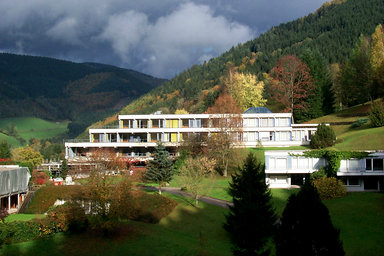
\includegraphics[width=3cm]{./../../common/images/photo_mfo.jpg}\\
Aplikacija SURFER je besplatna i mo\v ze se preuzeti na web stranici izlo\v zbe: 
\begin{center}
www.imaginary.org\\
\end{center}
 \vspace{0.2cm}
S desne strane mo\v zete odabrati jedno od poglavlja ovog tutoriala po\v cev\v si s plohom Limun. S lijeve strane mo\v zete odabrati neku drugu galeriju, npr.\ galeriju ploha fantasy.
\end{surferIntroPage}
